\documentclass[10pt,graphics,aspectratio=169,table]{beamer}
\usepackage{listings}
\usepackage{amsmath}
\usepackage{hyperref}
\usepackage{framed, color}
\usepackage{natbib}
\usepackage{csquotes}

\usetheme{metropolis}
\setbeamertemplate{bibliography item}[text]
\renewcommand{\bibsection}{}

\newcommand{\code}[0]{\lstinline[basicstyle=\ttfamily\color{white}]}
\newcommand{\cbox}[1]{\colorbox{black}{#1}}

\title{coffee101 - level up your coffee game}
\author{Emmanuel Diehl}
\date{ESE 2022}
\institute{NERD101 - ESE - ifsr - TU Dresden}

\titlegraphic{\hfill
\includegraphics[height=1.25cm]{logo}}
\begin{document}
\maketitle

\begin{frame}{Outline}
    \tableofcontents
\end{frame}

\section{Why you should not listen to me}

\begin{frame}{Taste is subjective}
\begin{itemize}
    \item "You're just jealous that they found happiness so much cheaper than you did." - Dankpods
    \item Tastebuds change towards bitter profiles with age 
    \item Desirable tastes vary with culture
    \item Emotion is more important than Extraction percentage
\end{itemize}


\centering
\end{frame}
\section{Ingredients}
\begin{frame}{Beans - Roasts}
\begin{tabular}{l|| c|c| c| p{6cm}}
    Roast: & Unroasted & light roast & medium roast & dark roast \\
    Taste:  & strong/sharp acidity & sweeter & caramel tones & Coal/burnt, no acidity \\
    Look: & green & yellow & brown, glistening, one crack & black, oily, two cracks\\
\end{tabular}   
\includegraphics[scale=0.02]{img/coffee bean.jpg}
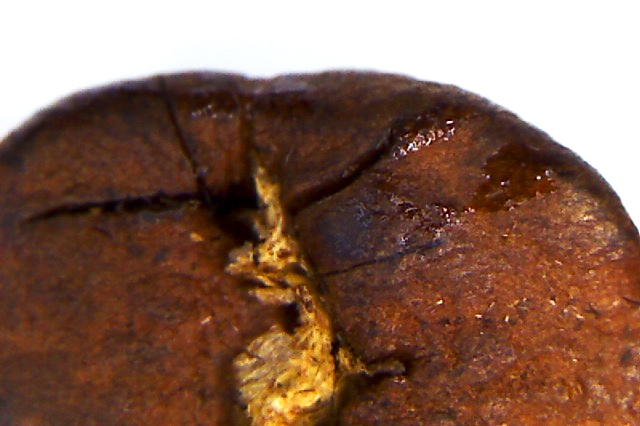
\includegraphics[scale=0.2]{img/Roasted-coffee-scorch-oil.jpg} \cite{roastingBean}
\end{frame}
\begin{frame}{Beans - Types}
\begin{itemize}
    \item Types of beans: 
    \begin{itemize}
        \item Arabica: most popular, mild taste
        \item Robusta: cheap, double the caffeine, sharp and woody taste
        \item Liberica: uncommon, sweet, fruity, floral
    \end{itemize}
    \item It is common to have Arabica/ Robusta blends between 1:1 to 9:1
    \item Decaffinated coffe is either sprayed with chemicals that burn while roasting or pre-boiled, so only darker roasts
    \end{itemize}
\end{frame}

\begin{frame}{Grinding beans}
    \begin{itemize}
        \item Roasted coffee oxidates, store airtight at 20-25 degrees
        \item Grinding espresso beans increases the surface by a factor of 10'000
        \item use withing two weeks
        \item Blade grinders get hot and grind unevenly
        \item Burr grinders are preferable (motor or hand powered)
    \end{itemize}
    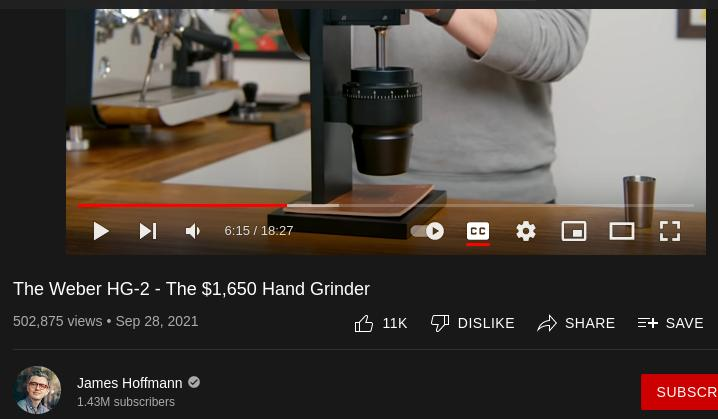
\includegraphics[scale=0.35]{img/Screenshot_handgrinder.jpg} \cite{expensiveGrinder}
\end{frame}

\begin{frame}{Grind  Size}
\begin{itemize}
    \item Extra coarse/ peppercorn size: cold brew or cowboy Coffee
    \item Coarse/ sea salt size: french press
    \item Medium coarse/ coarse sand: immersion brewing, clever drip
    \item Medium Grind/ smooth sand: Aeropress (3 min. brew), pour-over
    \item Medium fine grind/ fine sand: pour-over, aeropress (2-3 min. brew)
    \item Fine grind/ rough powder: espresso, mokka pot, aeropress (1 min. brew) 
    \item Extra fine/ flower: Turkish coffee
\end{itemize}
    
\end{frame}
\begin{frame}{Water}
    \begin{itemize}
        \item \text{ Water makes up 98\% of filter coffee and 93\% of espresso}
        \item Magnesium attracts acidic flavors from beans
        \item Calcium can cause limescale in machines (difficulty with flow, heating efficiency, damages)
        \item Consider experimenting with pre-boiling, descaling or filtering
    \end{itemize}
\end{frame}


\section{How to make coffee}

\begin{frame}{How to make Coffee}
    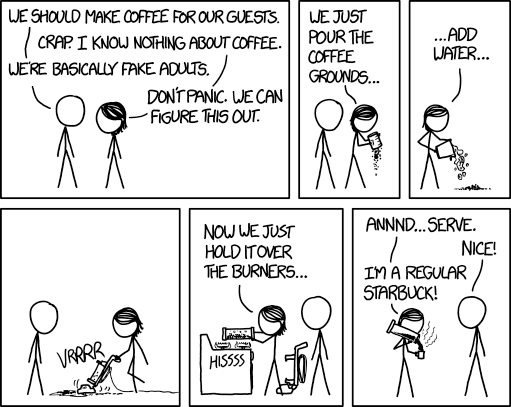
\includegraphics[scale=0.483]{img/coffeeXkcd.png} \cite{xkcd}
\end{frame}

\begin{frame}{Extraction - where the magic happens}
 \begin{itemize}
    \item Rough order of extraction:
    \begin{itemize}
      \item Caffeine
      \item Acids and fats
      \item Sugars
      \item Bitterness components
    \end{itemize}
    \item Influenced by temperature, pressure, surface area and time
    \item usually 91-94 degrees
 \end{itemize}
\end{frame}

\begin{frame}{Cold Brew - cheap, strong and refreshing (0-5€)}
    \begin{itemize}
        \item Usually medium - dark roasts
        \item Mix coarse, ground beans with cold water
        \item Let sit for 12 - 24 hours refrigerated or at room temperature
        \item Strain with cheesecloth, coffee filter or french press
        \item Flavor: little acidity, not too strong taste with low bitterness
        \item Tip 1: Mix 1:1 with milk/water, add ice and sweetener e.g. Agave syrup
        \item Tip 2: Snobs tell you it's a waste of good coffee because you don't extract complex acid profiles - don't listen to them
    \end{itemize}
\end{frame}

\begin{frame}{Moka - look like an Italian (10-40€}
    \begin{itemize}
        \item Medium - dark roasts to avoid acidity
        \item Fine grounds, a bit less than espresso
        \item Fill moka with water up to valve, add grounds to basket and place on heat until enough coffee is in the top chamber 
        \item Flavor: very concentrated, espresso style coffee (extracted at 1-2 bar vs 9 bar), no crema
        \item Tip: Use hot water for shorter extraction and avoid the "spewing phase"
    \end{itemize}
        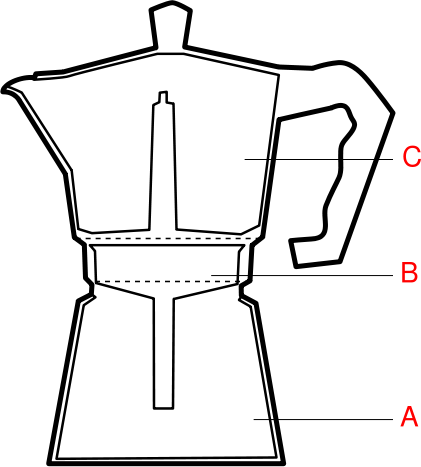
\includegraphics[scale=0.25]{img/421px-MokaCoffeePot.svg.png} \cite{mokaShematics}
        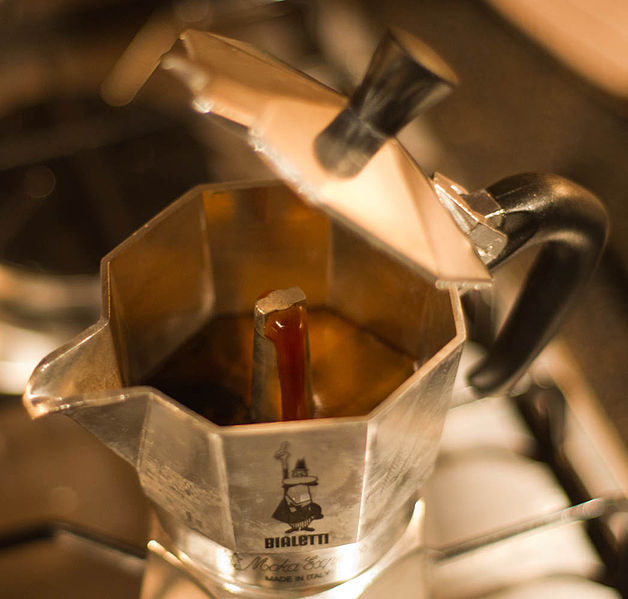
\includegraphics[scale=0.6]{img/628px-Moka_brewing.jpg} \cite{mokaBrewing}
\end{frame}

\begin{frame}{French Press (7-40€)}
    \begin{itemize}
        \item Coarse grind
        \item 1:12 coffee:water ratio
        \item Pour hot water on top and mix lightly (!)
        \item Wait four minutes, Press down plunger and pour
        \item Flavour: Full, no oils/fats lost in a filter. Sometimes some fine grounds
        \item Tip 1: Bloom with a 4th-6th of the water for 30 seconds, let sit for three and a half minutes
        \item Tip 2: Swirl hot water and discard it before you make the coffee to pre-heat it
    \end{itemize}
    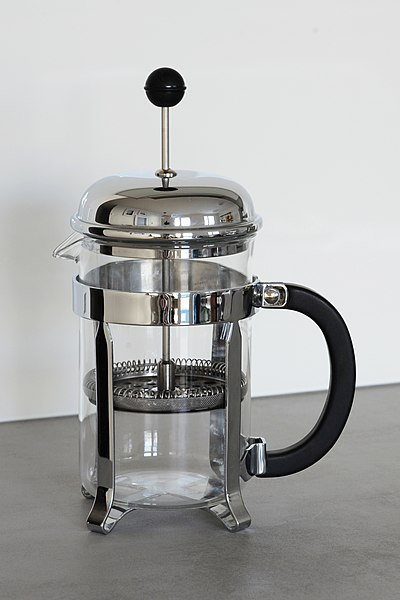
\includegraphics[scale=0.16]{img/400px-French_press_2020.jpg} \cite{frenchPress}
\end{frame}

\begin{frame}{Espresso - the pinnacle of coffee for pretentious purists (80-2000+€)}
\begin{itemize}
    \item Finely ground - medium, depending on the length of extraction
    \item Grounds are placed in a basket, distributed and pressed down with a tamp
    \item Basket sizes: solo, doppio/double and triplo with 7g, 14g and 21g
    \item Extraction length: ristretto/stretto (reduced), normale, lungo, caffee crema
    \item Serve in preheated glas/cup and stir gently
    \item Flavour: very intense - dilution might be desirable (water/milk/milk alternatives)
\end{itemize}
    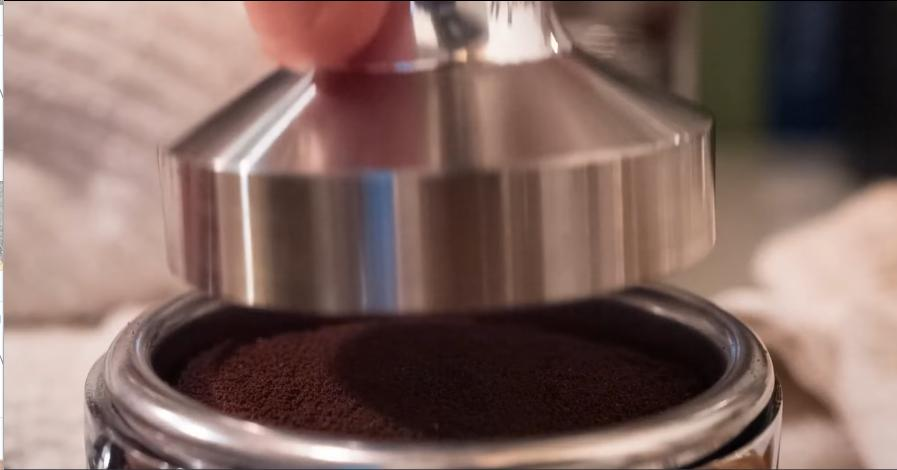
\includegraphics[scale=0.2]{img/Screenshot_2022-10-02_08-08-13.jpg} \cite{espresso}
    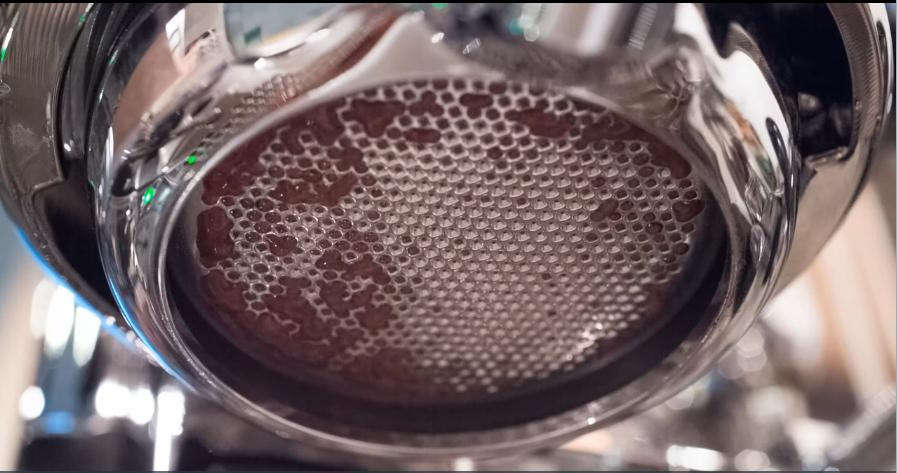
\includegraphics[scale=0.2]{img/Screenshot_2022-10-02_08-09-04.jpg} \cite{espresso}

\end{frame}

\begin{frame}{Espresso - Tips}
    \begin{itemize}
        \item Crema test - half a coffee spoon of sugar should be able to float on the crema for a bit
        \item Espresso machines can often be easily fixed up or bought used for cheap
        \item You can drink more if you pull smaller shots/decaf
        \item Make your own distribution tool with a cork and needles
        \item Try pulling a shot onto chocholate
    \end{itemize}
    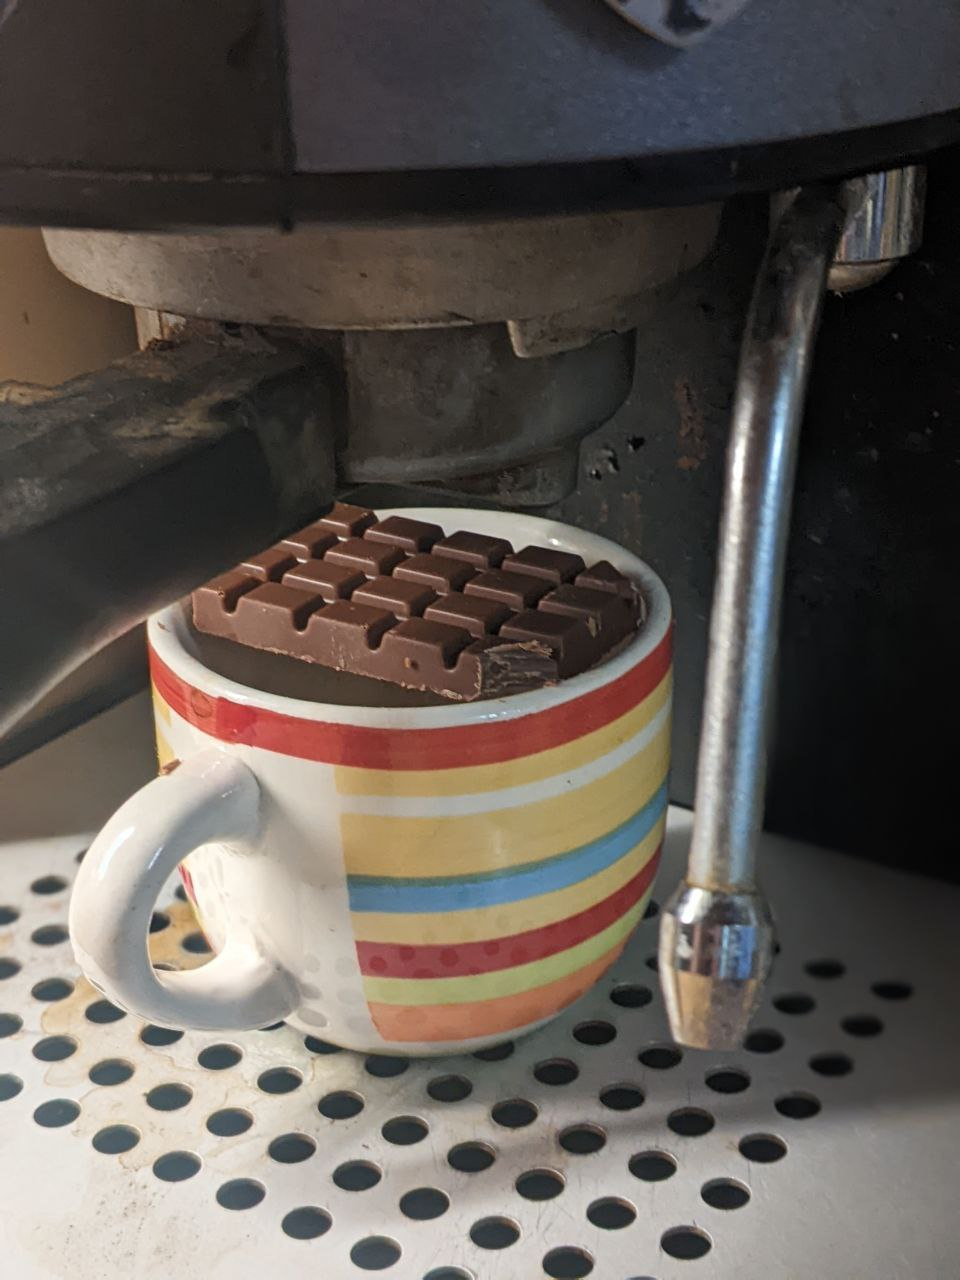
\includegraphics[scale =0.08]{img/chocolateShot.jpg} \cite{chocolate}
\end{frame}

\begin{frame}{Pour over (6-40€)}
    \begin{itemize}
        \item Place the pour over brewer on a cup or carafe. Add filter
        \item Fill a filter 2/3 - 3/4 with medium (coarse) grounds
        \item Add 50-70ml of hot water, stir and let bloom for 30-45 seconds
        \item Pour over the rest of the water in circles going in to evenly distribute it
        \item Flavour: Less rich, more singular due to removal of oil with paper filters
        \item Tip: Wet the filter before adding the coffee to get rid of any paper taste
        
    \end{itemize}
    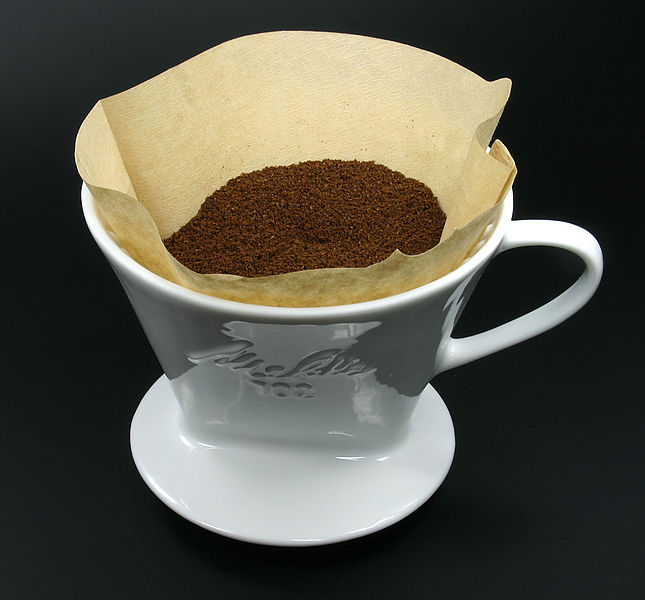
\includegraphics[scale=0.2]{img/645px-Kaffeefilter.jpg} \cite{pourOver}
\end{frame}

\section{Coffee and ethics}
\begin{frame}{Producers}
    \begin{itemize}
    \item 12 Million out of the 25 million coffee farmers (3.20 dollars/day) live below the international poverty line in Brazil alone
    \item Coffee plants are often treated with insecticides that can act as neurotoxins, cause cancer, miscarriages, etc. in farmers
    \item In various countries conditions similar to slavery and child labour are still present on some farms. Starbucks and Nestle are among the companies that sourced beans from those farms. \cite{reportBrazil}
\end{itemize}
\end{frame}


\begin{frame}[allowframebreaks]
        \frametitle{References}
        \bibliographystyle{ieeetr}
        \nocite{*}
        \bibliography{ref}
\end{frame}
\end{document}
